\chapter{Teorija brojeva}

\index{teorija brojeva}

\key{Teorija brojeva} je grana matematike
koja proučava cijele brojeve.
Teorija brojeva je fascinantno područje,
jer je mnoga pitanja o cijelim brojevima
vrlo teško riješiti čak i kada se
na prvi pogled čine jednostavnima.

Kao primjer, razmotrimo sljedeću jednadžbu:
\[x^3 + y^3 + z^3 = 33\]
Lako je pronaći tri realna broja $x$, $y$ i $z$
koji zadovoljavaju tu jednadžbu.
Na primjer, možemo odabrati
\[
\begin{array}{lcl}
x = 3, \\
y = \sqrt[3]{3}, \\
z = \sqrt[3]{3}.\\
\end{array}
\]
Međutim, otvoren je problem u teoriji brojeva
postoje li tri
\emph{cijela broja} $x$, $y$ i $z$
koja bi zadovoljavala tu jednadžbu \cite{bec07}.

U ovom poglavlju usredotočit ćemo se na osnovne pojmove
i algoritme u teoriji brojeva.
Kroz cijelo poglavlje pretpostavljat ćemo da su svi brojevi
cijeli, ako nije drukčije navedeno.

\section{Prosti brojevi i djelitelji}

\index{djeljivost}
\index{faktor}
\index{djelitelj}

Broj $a$ nazivamo \key{faktorom} ili \key{djeliteljem} broja $b$
ako $a$ dijeli $b$.
Ako je $a$ djelitelj broja $b$,
pišemo $a \mid b$, a inače pišemo $a \nmid b$.
Na primjer, djelitelji broja 24 su
1, 2, 3, 4, 6, 8, 12 i 24.

\index{prost broj}
\index{rastav na proste faktore}

Broj $n>1$ je \key{prost broj}
ako su njegovi jedini pozitivni djelitelji 1 i $n$.
Na primjer, 7, 19 i 41 su prosti brojevi,
ali 35 nije prost broj, jer je $5 \cdot 7 = 35$.
Za svaki broj $n>1$ postoji jedinstven
\key{rastav na proste faktore}
\[ n = p_1^{\alpha_1} p_2^{\alpha_2} \cdots p_k^{\alpha_k},\]
gdje su $p_1,p_2,\ldots,p_k$ različiti prosti brojevi, a
$\alpha_1,\alpha_2,\ldots,\alpha_k$ su pozitivni brojevi.
Na primjer, rastav broja 84 na proste faktore je
\[84 = 2^2 \cdot 3^1 \cdot 7^1.\]

\key{Broj djelitelja} broja $n$ jednak je
\[\tau(n)=\prod_{i=1}^k (\alpha_i+1),\]
jer za svaki prosti broj $p_i$ postoji
$\alpha_i+1$ načina da odaberemo koliko se puta
pojavljuje u djelitelju.
Na primjer, broj djelitelja
broja 84 je
$\tau(84)=3 \cdot 2 \cdot 2 = 12$.
Djelitelji su
1, 2, 3, 4, 6, 7, 12, 14, 21, 28, 42 i 84.

\key{Suma djelitelja} broja $n$ jednaka je
\[\sigma(n)=\prod_{i=1}^k (1+p_i+\ldots+p_i^{\alpha_i}) = \prod_{i=1}^k \frac{p_i^{a_i+1}-1}{p_i-1},\]
gdje se druga formula temelji na formuli za geometrijski niz.
Na primjer, suma djelitelja broja 84 je
\[\sigma(84)=\frac{2^3-1}{2-1} \cdot \frac{3^2-1}{3-1} \cdot \frac{7^2-1}{7-1} = 7 \cdot 4 \cdot 8 = 224.\]

\key{Proizvod djelitelja} broja $n$ jednak je
\[\mu(n)=n^{\tau(n)/2},\]
jer od djelitelja možemo formirati $\tau(n)/2$ parova,
od kojih svaki ima umnožak $n$.
Na primjer, djelitelji broja 84
tvore parove
$1 \cdot 84$, $2 \cdot 42$, $3 \cdot 28$, itd.,
pa je umnožak djelitelja $\mu(84)=84^6=351298031616$.

\index{savršen broj}

Broj $n$ nazivamo \key{savršenim brojem} ako je $n=\sigma(n)-n$,
tj. ako je $n$ jednak sumi svojih djelitelja
između $1$ i $n-1$.
Na primjer, 28 je savršen broj,
jer je $28=1+2+4+7+14$.

\subsubsection{Broj prostih brojeva}

Lako je pokazati da postoji beskonačno mnogo
prostih brojeva.
Kada bi prostih brojeva bilo konačno mnogo,
mogli bismo konstruirati skup $P=\{p_1,p_2,\ldots,p_n\}$
koji bi sadržavao sve proste brojeve.
Na primjer, $p_1=2$, $p_2=3$, $p_3=5$, i tako dalje.
Međutim, koristeći $P$, mogli bismo formirati novi prost broj
\[p_1 p_2 \cdots p_n+1\]
koji je veći od svih elemenata skupa $P$.
To je kontradikcija, pa prostih brojeva
mora biti beskonačno mnogo.

\subsubsection{Gustoća prostih brojeva}

Gustoća prostih brojeva govori nam kako često se prosti brojevi
pojavljuju među brojevima.
Neka $\pi(n)$ označava broj prostih brojeva između
$1$ i $n$. Na primjer, $\pi(10)=4$, jer
između $1$ i $10$ postoje 4 prosta broja: 2, 3, 5 i 7.

Moguće je pokazati da vrijedi
\[\pi(n) \approx \frac{n}{\ln n},\]
što znači da su prosti brojevi vrlo česti.
Na primjer, broj prostih brojeva između
$1$ i $10^6$ je $\pi(10^6)=78498$,
a $10^6 / \ln 10^6 \approx 72382$.

\subsubsection{Slutnje}

Postoji mnogo \emph{slutnji} o prostim brojevima.
Većina ljudi misli da su te slutnje istinite,
ali ih nitko još nije uspio dokazati.
Na primjer, sljedeće su slutnje poznate:

\begin{itemize}
\index{Goldbachova slutnja}
\item \key{Goldbachova slutnja}:
Svaki paran cijeli broj $n>2$ može se prikazati kao
suma $n=a+b$ tako da su i $a$ i $b$ prosti brojevi.
\index{prosti blizanci}
\item \key{Slutnja o prostim blizancima}:
Postoji beskonačno mnogo parova
oblika $\{p,p+2\}$,
gdje su i $p$ i $p+2$ prosti brojevi.
\index{Legendreova slutnja}
\item \key{Legendreova slutnja}:
Između brojeva $n^2$ i $(n+1)^2$ uvijek postoji
prost broj, gdje je $n$ bilo koji pozitivni cijeli broj.
\end{itemize}

\subsubsection{Osnovni algoritmi}

Ako broj $n$ nije prost,
može se prikazati kao umnožak $a \cdot b$,
gdje je $a \le \sqrt n$ ili $b \le \sqrt n$,
pa zasigurno ima djelitelja između $2$ i $\lfloor \sqrt n \rfloor$.
Koristeći to opažanje, možemo i provjeriti
je li broj prost i pronaći rastav broja
na proste faktore u $O(\sqrt n)$ vremenu.

Sljedeća funkcija \texttt{prime} provjerava
je li zadani broj $n$ prost.
Funkcija pokušava podijeliti $n$
svim brojevima između $2$ i $\lfloor \sqrt n \rfloor$,
i ako niti jedan od njih ne dijeli $n$, tada je $n$ prost.

\begin{lstlisting}
bool prime(int n) {
    if (n < 2) return false;
    for (int x = 2; x*x <= n; x++) {
        if (n%x == 0) return false;
    }
    return true;
}
\end{lstlisting}

\noindent
Sljedeća funkcija \texttt{factors}
konstruira vektor koji sadrži rastav
broja $n$ na proste faktore.
Funkcija dijeli $n$ njegovim prostim faktorima
i dodaje ih u vektor.
Postupak završava kada preostali broj $n$
više nema djelitelja između $2$ i $\lfloor \sqrt n \rfloor$.
Ako je $n>1$, on je prost i posljednji je faktor.

\begin{lstlisting}
vector<int> factors(int n) {
    vector<int> f;
    for (int x = 2; x*x <= n; x++) {
        while (n%x == 0) {
            f.push_back(x);
            n /= x;
        }
    }
    if (n > 1) f.push_back(n);
    return f;
}
\end{lstlisting}

Primijetimo da se svaki prosti faktor pojavljuje u vektoru
onoliko puta koliko dijeli taj broj.
Na primjer, $24=2^3 \cdot 3$,
pa je rezultat funkcije $[2,2,2,3]$.

\subsubsection{Eratostenovo sito}

\index{Eratostenovo sito}

\key{Eratostenovo sito}
%\footnote{Eratosthenes (c. 276 BC -- c. 194 BC) was a Greek mathematician.}
je algoritam predobrade
koji gradi niz pomoću kojega možemo
efikasno provjeriti je li zadani broj između $2 \ldots n$
prost i, ako nije, pronaći jedan njegov prosti faktor.

Algoritam gradi niz $\texttt{sieve}$
u kojem se koriste pozicije $2,3,\ldots,n$.
Vrijednost $\texttt{sieve}[k]=0$ znači
da je $k$ prost,
a vrijednost $\texttt{sieve}[k] \neq 0$
znači da $k$ nije prost i da je jedan
od njegovih prostih faktora $\texttt{sieve}[k]$.

Algoritam prolazi kroz brojeve
$2 \ldots n$ jedan po jedan.
Uvijek kada se pronađe novi prosti broj $x$,
algoritam zabilježi da višekratnici
broja $x$ ($2x,3x,4x,\ldots$) nisu prosti,
jer ih broj $x$ dijeli.

Na primjer, ako je $n=20$, niz izgleda ovako:

\begin{center}
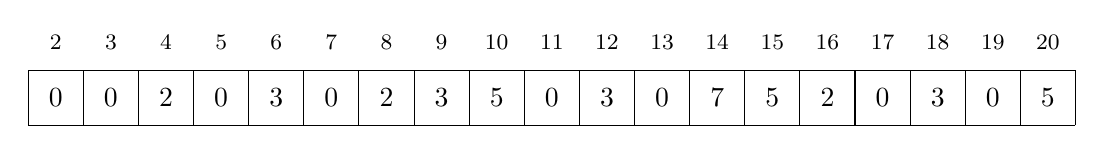
\begin{tikzpicture}[scale=0.7]
\draw (0,0) grid (19,1);

\node at (0.5,0.5) {$0$};
\node at (1.5,0.5) {$0$};
\node at (2.5,0.5) {$2$};
\node at (3.5,0.5) {$0$};
\node at (4.5,0.5) {$3$};
\node at (5.5,0.5) {$0$};
\node at (6.5,0.5) {$2$};
\node at (7.5,0.5) {$3$};
\node at (8.5,0.5) {$5$};
\node at (9.5,0.5) {$0$};
\node at (10.5,0.5) {$3$};
\node at (11.5,0.5) {$0$};
\node at (12.5,0.5) {$7$};
\node at (13.5,0.5) {$5$};
\node at (14.5,0.5) {$2$};
\node at (15.5,0.5) {$0$};
\node at (16.5,0.5) {$3$};
\node at (17.5,0.5) {$0$};
\node at (18.5,0.5) {$5$};

\footnotesize

\node at (0.5,1.5) {$2$};
\node at (1.5,1.5) {$3$};
\node at (2.5,1.5) {$4$};
\node at (3.5,1.5) {$5$};
\node at (4.5,1.5) {$6$};
\node at (5.5,1.5) {$7$};
\node at (6.5,1.5) {$8$};
\node at (7.5,1.5) {$9$};
\node at (8.5,1.5) {$10$};
\node at (9.5,1.5) {$11$};
\node at (10.5,1.5) {$12$};
\node at (11.5,1.5) {$13$};
\node at (12.5,1.5) {$14$};
\node at (13.5,1.5) {$15$};
\node at (14.5,1.5) {$16$};
\node at (15.5,1.5) {$17$};
\node at (16.5,1.5) {$18$};
\node at (17.5,1.5) {$19$};
\node at (18.5,1.5) {$20$};

\end{tikzpicture}
\end{center}

Sljedeći kod implementira Eratostenovo
sito.
Kod pretpostavlja da je svaki element
niza \texttt{sieve} u početku nula.

\begin{lstlisting}
for (int x = 2; x <= n; x++) {
    if (sieve[x]) continue;
    for (int u = 2*x; u <= n; u += x) {
        sieve[u] = x;
    }
}
\end{lstlisting}

Unutrašnja petlja algoritma izvršava se
$n/x$ puta za svaku vrijednost $x$.
Stoga je gornja ograda za vrijeme izvođenja
algoritma harmonijska suma
\[\sum_{x=2}^n n/x = n/2 + n/3 + n/4 + \cdots + n/n = O(n \log n).\]

\index{harmonijska suma}

Zapravo je algoritam efikasniji,
jer će se unutrašnja petlja izvršiti samo ako
je broj $x$ prost.
Može se pokazati da je vrijeme izvođenja
algoritma samo $O(n \log \log n)$,
složenost koja je vrlo blizu $O(n)$. 

\subsubsection{Euklidov algoritam}

\index{najveći zajednički djelitelj}
\index{najmanji zajednički višekratnik}
\index{Euklidov algoritam}

\key{Najveći zajednički djelitelj}
brojeva $a$ i $b$, $\gcd(a,b)$,
najveći je broj koji dijeli i $a$ i $b$,
a \key{najmanji zajednički višekratnik}
brojeva $a$ i $b$, $\textrm{lcm}(a,b)$,
najmanji je broj koji je djeljiv
i s $a$ i s $b$.
Na primjer,
$\gcd(24,36)=12$ i
$\textrm{lcm}(24,36)=72$.

Najveći zajednički djelitelj i najmanji zajednički višekratnik
povezani su na sljedeći način:
\[\textrm{lcm}(a,b)=\frac{ab}{\textrm{gcd}(a,b)}\]

\key{Euklidov algoritam}\footnote{Euklid je bio grčki matematičar koji
je živio oko 300. godine pr. Kr. Ovo je možda prvi poznati algoritam u povijesti.} pruža efikasan način
za pronalaženje najvećeg zajedničkog djelitelja dvaju brojeva.
Algoritam se temelji na sljedećoj formuli:
\begin{equation*}
    \textrm{gcd}(a,b) = \begin{cases}
               a        & b = 0\\
               \textrm{gcd}(b,a \bmod b) & b \neq 0\\
           \end{cases}
\end{equation*}

Na primjer,
\[\textrm{gcd}(24,36) = \textrm{gcd}(36,24)
= \textrm{gcd}(24,12) = \textrm{gcd}(12,0)=12.\]

Algoritam se može implementirati na sljedeći način:
\begin{lstlisting}
int gcd(int a, int b) {
    if (b == 0) return a;
    return gcd(b, a%b);
}
\end{lstlisting}

Može se pokazati da Euklidov algoritam radi
u $O(\log n)$ vremenu, gdje je $n=\min(a,b)$.
Najgori slučaj za algoritam je
slučaj kada su $a$ i $b$ uzastopni Fibonaccijevi brojevi.
Na primjer,
\[\textrm{gcd}(13,8)=\textrm{gcd}(8,5)
=\textrm{gcd}(5,3)=\textrm{gcd}(3,2)=\textrm{gcd}(2,1)=\textrm{gcd}(1,0)=1.\]

\subsubsection{Eulerova funkcija}

\index{relativno prosti}
\index{Eulerova funkcija}

Brojevi $a$ i $b$ su \key{relativno prosti}
ako je $\textrm{gcd}(a,b)=1$.
\key{Eulerova funkcija} $\varphi(n)$
%\footnote{Euler presented this function in 1763.}
daje broj brojeva između $1$ i $n$
koji su relativno prosti s $n$.
Na primjer, $\varphi(12)=4$,
jer su 1, 5, 7 i 11
relativno prosti s 12.

Vrijednost $\varphi(n)$ može se izračunati
iz rastava broja $n$ na proste faktore
pomoću formule
\[ \varphi(n) = \prod_{i=1}^k p_i^{\alpha_i-1}(p_i-1). \]
Na primjer, $\varphi(12)=2^1 \cdot (2-1) \cdot 3^0 \cdot (3-1)=4$.
Primijetimo da je $\varphi(n)=n-1$ ako je $n$ prost.

\section{Modularna aritmetika}

\index{modularna aritmetika}

U \key{modularnoj aritmetici}
skup brojeva je ograničen tako
da se koriste samo brojevi $0,1,2,\ldots,m-1$,
gdje je $m$ konstanta.
Svaki broj $x$
prikazan je brojem $x \bmod m$:
ostatkom nakon dijeljenja $x$ s $m$.
Na primjer, ako je $m=17$, tada je $75$
prikazan kao $75 \bmod 17 = 7$.

Često možemo uzeti ostatke prije nego provedemo
izračune.
Konkretno, vrijede sljedeće formule:
\[
\begin{array}{rcl}
(x+y) \bmod m & = & (x \bmod m + y \bmod m) \bmod m \\
(x-y) \bmod m & = & (x \bmod m - y \bmod m) \bmod m \\
(x \cdot y) \bmod m & = & (x \bmod m \cdot y \bmod m) \bmod m \\
x^n \bmod m & = & (x \bmod m)^n \bmod m \\
\end{array}
\]

\subsubsection{Modularno potenciranje}

Često se javlja potreba za efikasnim izračunom
vrijednosti $x^n \bmod m$.
To se može učiniti u $O(\log n)$ vremenu
koristeći sljedeću rekurziju:
\begin{equation*}
    x^n = \begin{cases}
               1        & n = 0\\
               x^{n/2} \cdot x^{n/2} & \text{$n$ je paran}\\
               x^{n-1} \cdot x & \text{$n$ je neparan}
           \end{cases}
\end{equation*}

Važno je da se u slučaju parnog $n$
vrijednost $x^{n/2}$ izračuna samo jednom.
To garantira da je vremenska složenost
algoritma $O(\log n)$, jer se $n$ uvijek prepolovi
kada je paran.

Sljedeća funkcija izračunava vrijednost
$x^n \bmod m$:

\begin{lstlisting}
int modpow(int x, int n, int m) {
    if (n == 0) return 1%m;
    long long u = modpow(x,n/2,m);
    u = (u*u)%m;
    if (n%2 == 1) u = (u*x)%m;
    return u;
}
\end{lstlisting}

\subsubsection{Fermatov teorem i Eulerov teorem}

\index{Fermatov teorem}
\index{Eulerov teorem}

\key{Fermatov teorem}
%\footnote{Fermat discovered this theorem in 1640.}
tvrdi da je
\[x^{m-1} \bmod m = 1\]
kada je $m$ prost te su $x$ i $m$ relativno prosti.
Iz toga također slijedi
\[x^k \bmod m = x^{k \bmod (m-1)} \bmod m.\]
Općenitije, \key{Eulerov teorem}
%\footnote{Euler published this theorem in 1763.}
tvrdi da je
\[x^{\varphi(m)} \bmod m = 1\]
kada su $x$ i $m$ relativno prosti.
Fermatov teorem slijedi iz Eulerovog teorema,
jer ako je $m$ prost, tada je $\varphi(m)=m-1$.

\subsubsection{Modularni inverz}

\index{modularni inverz}

Inverz broja $x$ modulo $m$
je broj $x^{-1}$ za koji vrijedi
\[ x x^{-1} \bmod m = 1. \]
Na primjer, ako je $x=6$ i $m=17$,
tada je $x^{-1}=3$, jer je $6\cdot3 \bmod 17=1$.

Koristeći modularne inverze, možemo dijeliti brojeve
modulo $m$, jer dijeljenje s $x$
odgovara množenju s $x^{-1}$.
Na primjer, da izračunamo vrijednost $36/6 \bmod 17$,
možemo koristiti izraz $2 \cdot 3 \bmod 17$,
jer je $36 \bmod 17 = 2$ i $6^{-1} \bmod 17 = 3$.

Međutim, modularni inverz ne postoji uvijek.
Na primjer, ako je $x=2$ i $m=4$, jednadžba
\[ x x^{-1} \bmod m = 1 \]
ne može se riješiti, jer su svi višekratnici broja 2
parni pa ostatak nikada ne može biti 1 kada je $m=4$.
Pokazuje se da se vrijednost $x^{-1} \bmod m$
može izračunati točno onda kada su $x$ i $m$ relativno prosti.

Ako modularni inverz postoji, može se
izračunati pomoću formule
\[
x^{-1} = x^{\varphi(m)-1}.
\]
Ako je $m$ prost, formula postaje
\[
x^{-1} = x^{m-2}.
\]
Na primjer,
\[6^{-1} \bmod 17 =6^{17-2} \bmod 17 = 3.\]

Ta nam formula omogućuje da efikasno izračunamo
modularne inverze koristeći algoritam modularnog potenciranja.
Formula se može izvesti pomoću Eulerovog teorema.
Prvo, modularni inverz mora zadovoljavati sljedeću jednadžbu:
\[
x x^{-1} \bmod m = 1.
\]
S druge strane, prema Eulerovom teoremu,
\[
x^{\varphi(m)} \bmod m =  xx^{\varphi(m)-1} \bmod m = 1,
\]
pa su brojevi $x^{-1}$ i $x^{\varphi(m)-1}$ jednaki.

\subsubsection{Računalna aritmetika}

U programiranju su cijeli brojevi bez predznaka prikazani modulo $2^k$,
gdje je $k$ broj bitova tipa podatka.
Uobičajena posljedica toga je da se broj prelije
ako postane prevelik.

Na primjer, u C++-u su brojevi tipa \texttt{unsigned int}
prikazani modulo $2^{32}$.
Sljedeći kod deklarira varijablu tipa
\texttt{unsigned int} čija je vrijednost $123456789$.
Nakon toga se ta vrijednost množi sama sobom,
a rezultat je
$123456789^2 \bmod 2^{32} = 2537071545$.

\begin{lstlisting}
unsigned int x = 123456789;
cout << x*x << "\n"; // 2537071545
\end{lstlisting}

\section{Rješavanje jednadžbi}

\subsubsection*{Diofantske jednadžbe}

\index{Diofantska jednadžba}

\key{Diofantska jednadžba}
%\footnote{Diophantus of Alexandria was a Greek mathematician who lived in the 3th century.}
je jednadžba oblika
\[ ax + by = c, \]
gdje su $a$, $b$ i $c$ konstante,
a treba pronaći vrijednosti $x$ i $y$.
Svaki broj u jednadžbi mora biti cijeli broj.
Na primjer, jedno rješenje jednadžbe
$5x+2y=11$ je $x=3$ i $y=-2$.

\index{prošireni Euklidov algoritam}

Diofantsku jednadžbu možemo efikasno riješiti
koristeći Euklidov algoritam.
Pokazuje se da Euklidov algoritam možemo proširiti
tako da pronađe brojeve $x$ i $y$
koji zadovoljavaju sljedeću jednadžbu:
\[
ax + by = \textrm{gcd}(a,b)
\]

Diofantska jednadžba može se riješiti ako je
$c$ djeljiv s
$\textrm{gcd}(a,b)$, a
inače se ne može riješiti.

Kao primjer, pronađimo brojeve $x$ i $y$
koji zadovoljavaju sljedeću jednadžbu:
\[
39x + 15y = 12
\]
Jednadžba se može riješiti, jer je
$\textrm{gcd}(39,15)=3$ i $3 \mid 12$.
Kada Euklidov algoritam izračunava
najveći zajednički djelitelj brojeva 39 i 15,
daje sljedeći niz poziva funkcije:
\[
\textrm{gcd}(39,15) = \textrm{gcd}(15,9)
= \textrm{gcd}(9,6) = \textrm{gcd}(6,3)
= \textrm{gcd}(3,0) = 3 \]
To odgovara sljedećim jednadžbama:
\[
\begin{array}{lcl}
39 - 2 \cdot 15 & = & 9 \\
15 - 1 \cdot 9 & = & 6 \\
9 - 1 \cdot 6 & = & 3 \\
\end{array}
\]
Koristeći te jednadžbe, možemo izvesti
\[
39 \cdot 2 + 15 \cdot (-5) = 3
\]
a množenjem toga s 4 rezultat je
\[
39 \cdot 8 + 15 \cdot (-20) = 12,
\]
pa je rješenje jednadžbe
$x=8$ i $y=-20$.

Rješenje Diofantske jednadžbe nije jedinstveno,
jer možemo formirati beskonačno mnogo rješenja
ako znamo jedno rješenje.
Ako je par $(x,y)$ rješenje, tada su i svi parovi
\[(x+\frac{kb}{\textrm{gcd}(a,b)},y-\frac{ka}{\textrm{gcd}(a,b)})\]
rješenja, gdje je $k$ bilo koji cijeli broj.

\subsubsection{Kineski teorem o ostacima}

\index{Kineski teorem o ostacima}

\key{Kineski teorem o ostacima} rješava
skup jednadžbi oblika
\[
\begin{array}{lcl}
x & = & a_1 \bmod m_1 \\
x & = & a_2 \bmod m_2 \\
\cdots \\
x & = & a_n \bmod m_n \\
\end{array}
\]
gdje su svi parovi brojeva $m_1,m_2,\ldots,m_n$ relativno prosti.

Neka je $x^{-1}_m$ inverz broja $x$ modulo $m$, i
\[ X_k = \frac{m_1 m_2 \cdots m_n}{m_k}.\]
Koristeći tu notaciju, rješenje tih jednadžbi je
\[x = a_1 X_1 {X_1}^{-1}_{m_1} + a_2 X_2 {X_2}^{-1}_{m_2} + \cdots + a_n X_n {X_n}^{-1}_{m_n}.\]
U tom rješenju, za svaki $k=1,2,\ldots,n$,
\[a_k X_k {X_k}^{-1}_{m_k} \bmod m_k = a_k,\]
jer je
\[X_k {X_k}^{-1}_{m_k} \bmod m_k = 1.\]
Kako su svi ostali članovi u sumi djeljivi s $m_k$,
oni ne utječu na ostatak,
pa je $x \bmod m_k = a_k$.

Na primjer, rješenje za
\[
\begin{array}{lcl}
x & = & 3 \bmod 5 \\
x & = & 4 \bmod 7 \\
x & = & 2 \bmod 3 \\
\end{array}
\]
je
\[ 3 \cdot 21 \cdot 1 + 4 \cdot 15 \cdot 1 + 2 \cdot 35 \cdot 2 = 263.\]

Nakon što pronađemo rješenje $x$,
možemo stvoriti beskonačno mnogo drugih rješenja,
jer su svi brojevi oblika
\[x+m_1 m_2 \cdots m_n\]
također rješenja.

\section{Ostali rezultati}

\subsubsection{Lagrangeov teorem}

\index{Lagrangeov teorem}

\key{Lagrangeov teorem}
%\footnote{J.-L. Lagrange (1736--1813) was an Italian mathematician.}
tvrdi da se svaki pozitivni cijeli broj
može prikazati kao suma četiriju kvadrata, tj.
$a^2+b^2+c^2+d^2$.
Na primjer, broj 123 može se prikazati
kao suma $8^2+5^2+5^2+3^2$.

\subsubsection{Zeckendorfov teorem}

\index{Zeckendorfov teorem}
\index{Fibonaccijev broj}

\key{Zeckendorfov teorem}
%\footnote{E. Zeckendorf published the theorem in 1972 \cite{zec72}; however, this was not a new result.}
tvrdi da svaki
pozitivni cijeli broj ima jedinstven prikaz
kao suma Fibonaccijevih brojeva takva da
nikoja dva broja nisu jednaka ni uzastopna
Fibonaccijeva broja.
Na primjer, broj 74 može se prikazati
kao suma $55+13+5+1$.

\subsubsection{Pitagorine trojke}

\index{Pitagorina trojka}
\index{Euklidova formula}

\key{Pitagorina trojka} je trojka $(a,b,c)$
koja zadovoljava Pitagorin teorem
$a^2+b^2=c^2$, što znači da postoji pravokutni trokut
s duljinama stranica $a$, $b$ i $c$.
Na primjer, $(3,4,5)$ je Pitagorina trojka.

Ako je $(a,b,c)$ Pitagorina trojka,
sve trojke oblika $(ka,kb,kc)$
također su Pitagorine trojke, gdje je $k>1$.
Pitagorina trojka je \emph{primitivna} ako su
$a$, $b$ i $c$ relativno prosti,
a sve Pitagorine trojke mogu se konstruirati
iz primitivnih trojki pomoću množitelja $k$.

\key{Euklidova formula} može se koristiti za dobivanje
svih primitivnih Pitagorinih trojki.
Svaka takva trojka je oblika
\[(n^2-m^2,2nm,n^2+m^2),\]
gdje je $0<m<n$, $n$ i $m$ su relativno prosti
i barem jedan od $n$ i $m$ je paran.
Na primjer, kada je $m=1$ i $n=2$, formula
daje najmanju Pitagorinu trojku
\[(2^2-1^2,2\cdot2\cdot1,2^2+1^2)=(3,4,5).\]

\subsubsection{Wilsonov teorem}

\index{Wilsonov teorem}

\key{Wilsonov teorem}
%\footnote{J. Wilson (1741--1793) was an English mathematician.}
tvrdi da je broj $n$
prost točno onda kada je
\[(n-1)! \bmod n = n-1.\]
Na primjer, broj 11 je prost, jer je
\[10! \bmod 11 = 10,\]
a broj 12 nije prost, jer je
\[11! \bmod 12 = 0 \neq 11.\]

Stoga se Wilsonov teorem može koristiti za utvrđivanje
je li broj prost. Međutim, u praksi se teorem ne može
primijeniti na velike vrijednosti $n$, jer je teško
izračunati vrijednosti $(n-1)!$ kada je $n$ velik.


